\documentclass[aspectratio=169]{beamer}
\usetheme{simple}

\input{preamble/preamble.tex}
\input{preamble/preamble_math.tex}
% \input{preamble/preamble_acronyms.tex}

\title{STATS305B: Applied Statistics II}
\subtitle{Poisson processes}
\author{Scott Linderman}
\date{\today}



\begin{document}


\maketitle


\begin{frame}{Course Outline}

\begin{itemize}
    \item Weeks 1-3: Classics: Exponential family distributions and GLMs
    \item Weeks 4-5: Bayesian Inference algorithms: MCMC and variational inference
    \item Weeks 6-7: Latent variable models: mixture models, HMMs, etc.
    \item Weeks 8-9: Deep generative models: VAEs, Transformers, Deep SSMs, Denoising diffusion models
    \item Week 10: Stochastic Process Models
\end{itemize}

\end{frame}


\begin{frame}{Learning Objectives}
    \begin{itemize}
    \item Understand the mathematical underpinnings of \textbf{classical and modern models for discrete data}.
    
    \item Develop expertise in an array of \textbf{algorithms for parameter estimation and inference} in these models.
    
    \item Be able to code these models and algorithms \textbf{from scratch in Python}.
    \end{itemize}
\end{frame}

\begin{frame}{Assignments}

\begin{itemize}
\item Weeks 1-3: Classics: Exponential family distributions and GLMs \\
\qquad \textit{Predict outcomes of college football games with a Bradley-Terry model.}

\item Weeks 4-5: Bayesian Inference algorithms: MCMC and variational inference \\
\qquad \textit{Election forecasting with a Bayesian GLM.}

\item Weeks 6-7: Latent variable models: mixture models, HMMs, etc. \\
\qquad \textit{Changepoint detection in time series data.}

\item Weeks 8-9: Deep generative models: VAEs, Transformers, Deep SSMs, Denoising diffusion models \\
\qquad \textit{Build a small LLM.}

\item Week 10: Stochastic Process Models
\end{itemize}
\end{frame}
    

\begin{frame}{Outline}
\begin{itemize}
    \item Defining properties of a Poisson process
    \item Four ways to sample a Poisson process
    \item Beyond Poisson: Hawkes processes 
\end{itemize}
\end{frame}

\begin{frame}{Defining properties of a Poisson process}
    \begin{columns}
    \begin{column}{.55\textwidth}
    \begin{itemize}
        \itemsep1em
        
        \item Poisson processes are \textbf{stochastic processes} that generate \textbf{random sets of points} $\{\mbx_n\}_{n=1}^N \subset \cX$.
        
        \item Poisson processes are governed by an \textbf{intensity function}, $\lambda(\mbx): \cX \to \reals_+$.
        
        \item<2->\textbf{Property \#1:} The number of points in any interval is a Poisson random variable,
        \begin{align}
            N(\cA) &\sim \distPoisson\left(\int_{\cA} \lambda(\mbx) \dif \mbx \right) 
        \end{align}
        
        \item<3->\textbf{Property \#2:} Disjoint intervals are independent,
        \begin{align}
            N(\cA) \independent N(\cB) \iff \cA \cap \cB = \varnothing
        \end{align}
    \end{itemize}
    \end{column}
    \begin{column}{.45\textwidth}
    \begin{figure}
        \centering
        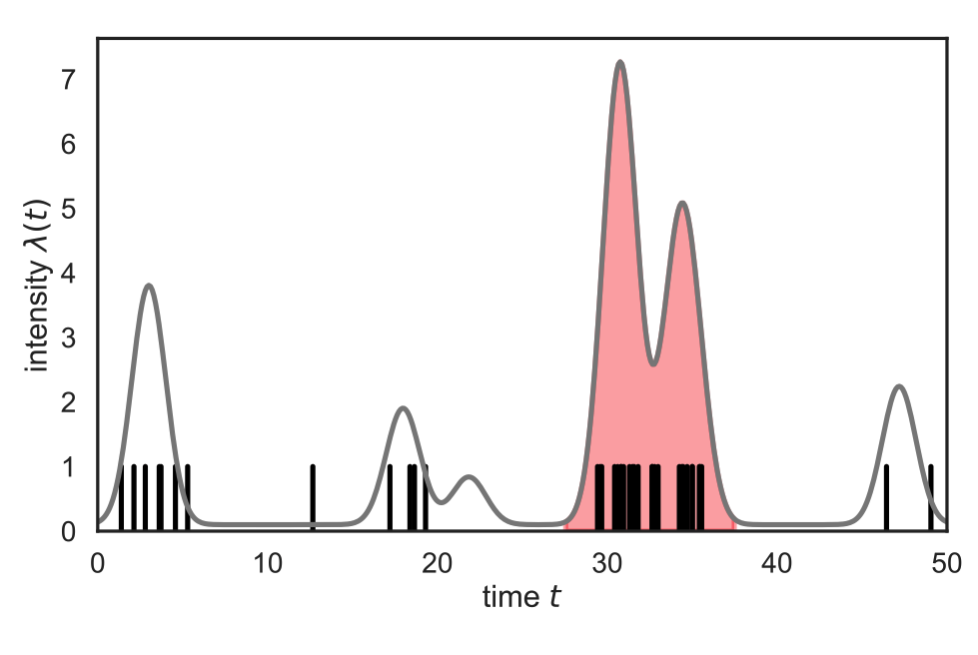
\includegraphics[width=\linewidth]{17_poisson_processes//poisson_process.png}
    \end{figure}
    \end{column}
    \end{columns}
\end{frame}

\begin{frame}{Example applications of Poisson processes}
    \begin{itemize}
        \item Modeling neural firing rates
        \item Locations of trees in a forest
        \item Locations of stars in astronomical surveys
        \item Arrival times of customers in a queue (or HTTP requests to a server)
        \item Locations of bombs in London during World War II
        \item Times of photon detections on a light sensor
        \item Others?
    \end{itemize}
\end{frame}

\begin{frame}{Four ways to sample a Poisson process}
\begin{enumerate}
    \item The top-down approach
    \item The interval approach
    \item The time-rescaling approach
    \item The thinning approach
\end{enumerate}    
\end{frame}

\begin{frame}{Top-down sampling of a Poisson process}
    Given $\lambda(\mbx)$ (and a domain $\cX$):
    \begin{enumerate}
        \itemsep1em
        \item Sample the \textbf{total number of points} 
        \begin{align}
            N &\sim \distPoisson \left( \int_{\cX} \lambda(\mbx) \dif \mbx \right)
        \end{align}
        
        \item Sample the \textbf{locations} of the points
        \begin{align}
            \mbx_n &\iid{\sim} \frac{\lambda(\mbx)}{\int_{\cX} \lambda(\mbx') \dif \mbx'}
        \end{align}
        for $n=1,\ldots,N$.
    \end{enumerate}
    \textbf{Question: } what assumptions are necessary for this procedure to be tractable?
\end{frame}

\begin{frame}[t]{Deriving the Poisson process likelihood}
    \textbf{Exercise: } from the top-down sampling process, derive the Poisson process likelihood,
    \begin{align}
        p\left(\{\mbx_n\}_{n=1}^N \mid \lambda(\mbx) \right) = \hspace{30em}
    \end{align}
\end{frame}

\begin{frame}{Intervals of a homogeneous Poisson process}
    \begin{itemize}
        \itemsep1em
        
        \item A Poisson process is \textbf{homogeneous} if its intensity is constant, $\lambda(\mbx) \equiv \lambda$.
        
        \item<2->\textbf{Property \#3:} A homogeneous Poisson process on $[0, T] \subset \reals$ (e.g. where points correspond to arrival times) has \textbf{independent, exponentially distributed intervals},
        \begin{align}
            \Delta_n = x_n - x_{n-1} &\iid{\sim} \mathrm{Exp}(\lambda)
        \end{align}
        
        \item<3-> \textbf{Property \#4:} A homogeneous Poisson process is \textbf{memoryless} --- the amount of time until the next point arrives is independent of the time elapsed since the previous point arrived.
    \end{itemize}
\end{frame}

\begin{frame}{Sampling a homogeneous Poisson process by simulating intervals}
We can sample a homogeneous Poisson process on $[0, T]$ by simulating intervals as follows:
\begin{enumerate}
    \item Initialize $\mbX = \varnothing$ and $x_0 = 0$
    \item For $n=1, 2, \ldots$:
    \begin{itemize}
        \item Sample $\Delta_n \sim \mathrm{Exp}(\lambda)$.
        \item Set $x_n = x_{n-1} + \Delta_n$.
        \item If $x_n > T$, break and return $\mbX$,
        \item Else, set $\mbX \leftarrow \mbX \cup \{x_n\}$.
    \end{itemize}
\end{enumerate}
\end{frame}

\begin{frame}[t]{Deriving the likelihood of a homogeneous Poisson process}
    \textbf{Exercise:} from the interval sampling process, derive the likelihood of a homogeneous Poisson process. Show that it is the same as what you derived from the top-down sampling process.
\end{frame}

\begin{frame}{Sampling an inhomogeneous Poisson process by time-rescaling}
    \begin{itemize}
        \itemsep1em
        \item Now consider an \textbf{inhomogeneous} Poisson process on $[0, T]$; i.e. one with a non-constant intensity.
        
        \item<2-> Apply the change of variables,
        \begin{align}
            x &\mapsto \int_0^x \lambda(t) \dif t \triangleq \Lambda(x)
        \end{align}
        Note that this is an \textbf{invertible transformation} when $\lambda(x) > 0$. 
        
        \item<3-> Sample a homogeneous Poisson process with unit rate on $[0, \Lambda(T)]$ to get points $\mbU = \{u_n\}_{n=1}^N$. Then set,
        \begin{align}
            \mbX &= \{\Lambda^{-1}(u_n): u_n \in \mbU\}.
        \end{align}
        
        \item<4-> \textbf{Sanity check:} what is the expected value of $N$?
    \end{itemize}
\end{frame}

\begin{frame}[t]{Sampling an inhomogeneous Poisson process by time-rescaling, in pictures}
    \textbf{Note:} this is the analog of \textbf{inverse-CDF} sampling.
\end{frame}

\begin{frame}[t]{A Goodness of fit test for inhomogeneous Poisson processes}
    \begin{itemize}
        \itemsep1em
        
        \item \citet{brown2002time} used the time-rescaling sampling procedure to develop a goodness-of-fit test for inhomogeneous Poisson processes.
        
        \item<2-> Suppose you observe a set of points $\{x_n\}_{n=1}^N \subset [0,T]$ and you want to test whether they are well-modeled by an inhomogeneous Poisson process with rate $\lambda(x)$. 
        
        \item<3-> Let $\Delta_n = \Lambda(x_n) - \Lambda(x_{n-1}$) with $\Lambda(x_0) =0$. If the model is a good fit, then $\Delta_n \iid{\sim} \mathrm{Exp}(1)$.
        
        \item<4-> Perform a further transformation $z_n = 1 - e^{-\Delta_n}$. Then $z_n \iid{\sim} \mathrm{Unif}([0, 1])$.
        
        \item<5-> Now sort the $z_n$'s in increasing order into $(z_{(1)}, \ldots, z_{(N)})$, so $z_{(1)}$ is the smallest value.
        
        \item<6-> Intuitively, the points $\big(\tfrac{n-1/2}{N}, z_{(n)}\big)$ should like along a 45$^\circ$ line.
    \end{itemize}
\end{frame}

\begin{frame}{A Goodness of fit test for inhomogeneous Poisson processes II}
\begin{columns}
\begin{column}{0.6\textwidth}
    \begin{itemize}
        \itemsep1em
        
        \item We can check for significant departures from the 45$^\circ$ line using a simple visual test. 
        
        \item The order statistics $z_{(n)}$ are marginally beta distributed,
        \begin{align}
            z_{(n)} &\sim \mathrm{Beta}(n, N-n+1)
        \end{align}
        The mean is $\tfrac{n}{N+1}$ and its mode is $\tfrac{n-1}{N-1}$.
        
        \item Then, use the 2.5\% and 97.5\% quantiles of the beta distribution to obtain confidence intervals around the 45$^\circ$ line.
    \end{itemize}
\end{column}
\begin{column}{.4\textwidth}
\begin{figure}
    \centering
    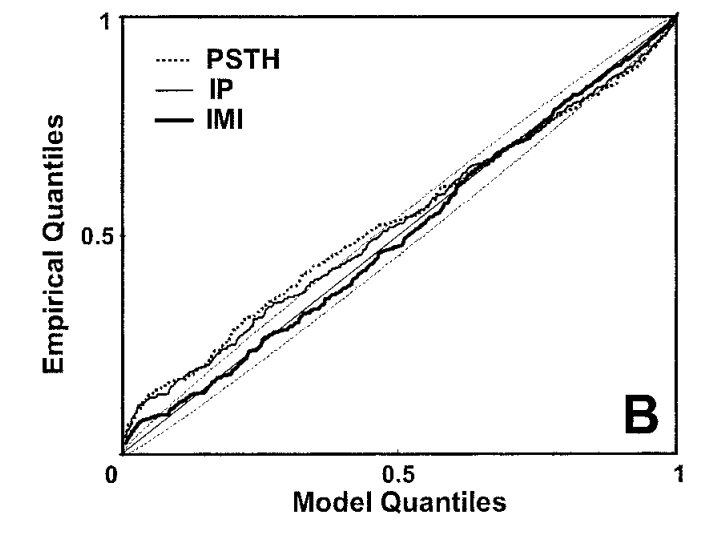
\includegraphics[width=\linewidth]{17_poisson_processes//qq_plot.png}
    \caption{Figure 1 from~\citet{brown2002time}.}
\end{figure}
\end{column}
\end{columns}
\end{frame}

\begin{frame}{The Poisson Superposition Principle}
    \begin{itemize}
        \itemsep1em
        \item<1-> \textbf{Property \#5:}  The union (a.k.a. superposition) of independent Poisson processes is also a Poisson process.
        
        \item<2-> Suppose we have two independent Poisson processes on the same domain $\cX$,
        \begin{align}
            \{\mbx_n\}_{n=1}^N &\sim \mathrm{PP}(\lambda_1(\mbx)) \\
            \{\mbx'_m\}_{m=1}^M &\sim \mathrm{PP}(\lambda_2(\mbx))
        \end{align}
        Then
        \begin{align}
            \{\mbx_n\}_{n=1}^N \cup \{\mbx'_m\}_{m=1}^M &\sim \mathrm{PP}(\lambda_1(\mbx) + \lambda_2(\mbx))
        \end{align}
        
        \item<3->This is the analog of the fact that the sum of independent Poisson random variables is Poisson.
    \end{itemize}
\end{frame}

\begin{frame}{Poisson thinning}
\begin{itemize}
    \itemsep1em
    
    \item The opposite of Poisson superposition is \textbf{Poisson thinning}. 
    
    \item Suppose we have points $\{\mbx_n\}_{n=1}^N \sim \mathrm{PP}(\lambda(\mbx))$ where $\lambda(\mbx) = \lambda_1(\mbx) + \lambda_2(\mbx)$.
    
    \item Sample independent binary variables 
    \begin{align}
        z_n \sim \mathrm{Bern}\left(\frac{\lambda_1(\mbx_n)}{\lambda_1(\mbx_n) + \lambda_2(\mbx_n)} \right).
    \end{align}
    
    \item Then $\{\mbx_n: z_n = 1\} \sim \mathrm{PP}(\lambda_1(\mbx))$ and $\{\mbx_n: z_n = 0\} \sim \mathrm{PP}(\lambda_2(\mbx))$.
\end{itemize}
\end{frame}

\begin{frame}[t]{Sampling a Poisson process by thinning}
\textbf{Exercise:} Use Poisson thinning to sample an inhomogeneous Poisson process with a bounded intensity,~$\lambda(\mbx) \leq \lambda_{\mathsf{max}}$.

\textbf{Question:} What Monte Carlo sampling method is this akin to?
\end{frame}

\begin{frame}{Outline}
\begin{itemize}
    \item Defining properties of a Poisson process
    \item Four ways to sample a Poisson process
    \item \textbf{Beyond Poisson: Hawkes Processes}
\end{itemize}
\end{frame}

\begin{frame}{What's not to love about Poisson processes?}
    
\end{frame}

\begin{frame}{Conditional intensity functions}
\begin{itemize}
    \itemsep1em 
    
    \item One way of introducing dependence is via an \textbf{autoregressive model}. Consider a point process on a time interval $[0, T]$.
    
    \item<2-> Let $\lambda(t \mid \cH_t)$ denote a \textbf{conditional intensity function} where $\cH_t$ is the \textbf{history} of points before time $t$. 
    
    \item<3-> Technically, $\cH_t$ is a \textbf{filtration} in the language of stochastic processes.
    
    \item<4-> Allowing past points to influence the intensity function enables more complex, non-Poisson models.
\end{itemize}
\end{frame}

\begin{frame}{Hawkes processes}
\begin{itemize}
    \itemsep1em 
    
    \item Hawkes processes~\citep{hawkes1971spectra} are \textbf{self-exciting point processes}.
    
    \item<2-> Their conditional intensity function is modeled as,
    \begin{align}
        \lambda(t \mid \cH_t) &= \lambda_0 + \sum_{t_n \in \cH_t} h(t - t_n),
    \end{align}
    where $h: \reals_+ \mapsto \reals_+$ is a positive \textbf{impulse response} or \textbf{influence function}.
    
    \item<3-> For example, the impulse responses could be modeled as exponential functions,
    \begin{align}
        h(\Delta t) &= \tfrac{w}{\tau} e^{-\tfrac{\Delta t}{\tau}} = w \cdot \mathrm{Exp}(\Delta t; \tau),
    \end{align}
    where $\tau \in \reals_+$ is a time-constant governing the rate of decay and $w \in \reals_+$ is a scaling parameter such that~$\int_0^\infty h(\Delta t) \dif \Delta t = w$.
\end{itemize}
\end{frame}

\begin{frame}{Hawkes processes, in pictures}
    
\end{frame}

\begin{frame}[t, allowframebreaks]{Maximum likelihood estimation for Hawkes processes}
\begin{itemize}
    \itemsep1em
    
    \item Suppose we observe a collection of time points $\{t_n\}_{n=1}^N \subset [0, T]$ and want to estimate the parameters $\mbtheta = (\lambda_0, w)$ of a Hawkes process with an exponential impulse response function. (Consider $\tau$ to be fixed.)
    
    \item The Hawkes process log likelihood is just like that of a Poisson process,
    \begin{align}
        \log p(\{t_n\}_{n=1}^N \mid \mbtheta) &= -\int_0^T \lambda_{\mbtheta}(t \mid \cH_t) \dif t + \sum_{n=1}^N \log \lambda_{\mbtheta}(t_n \mid \cH_t)
    \end{align}
    
    \item Substituting in the form of the conditional intensity, we can simplify the log likelihood to,
    \begin{align}
        \nonumber
        \log p(\{t_n\}_{n=1}^N \mid \mbtheta) &=
        -\int_0^T \Big[\lambda_0 + w\sum_{t_n \in \cH_t} \mathrm{Exp}(t-t_n; \tau) \dif t \Big] \\
        &\hspace{8em}+ \sum_{n=1}^N \log \Big(\lambda_0 + w \sum_{t_m \in \cH_{t_n}} \mathrm{Exp}(t_n - t_m; \tau) \Big) \\
        &\approx 
        -\mbtheta^\top \mbphi_0 + \sum_{n=1}^N \log \Big(\mbtheta^\top \mbphi_n \Big)
    \end{align}
    where $\mbphi_0 = (T, N)^\top$ and  $\mbphi_n = \Big(1, \, \sum_{t_m \in \cH_{t_n}} \mathrm{Exp}(t_n - t_m; \tau) \Big)^\top$.
    
    \item \textbf{Questions: } What approximation did we make? How would you maximize the log likelihood as a function of $\mbtheta$?
\end{itemize}
\end{frame}

\begin{frame}[t,allowframebreaks]{Nonlinear Hawkes processes}

Hawkes processes only allow for excitatory impulse responses ($w \in \reals_+$). What if we want to model \textbf{self-inhibitory} influences as well? A natural generalization of the Hawkes process is,
\begin{align*}
\lambda(t \mid \cH_t) &= f(\beta_0 + \beta \sum_{t_n \in \cH_t} g(t - t_n))
\end{align*}
where $f: \reals \mapsto \reals_+$ is a rectifying nonlinear function and $\beta_0, \beta \in \reals$ can be positive or negative.

These models are a bit more challenging because the Poisson process likelihood requires the integrated intesity function, which is generally intractable. 
Instead, we can approximate the integral with a Riemann sum,
\begin{align*}
\int \lambda(t \mid \cH_t) \dif t &\approx \sum_{i=0}^{\lfloor {T}/{\Delta}\rfloor - 1} \lambda(i \Delta \mid \cH_{i \Delta}) \Delta
\end{align*}
which essentially treats the intensity as piecewise constant within each interval of length $\Delta$. 

In that approximation, the Poisson process likelihood is equivalent, up to a scale factor, to a product of Poisson likelihoods,
\begin{align*}
p(\{t_n\}_{n=1}^N) &\approx
\prod_{i=0}^{\lfloor {T}/{\Delta}\rfloor - 1} \mathrm{Po}(N_i \mid \lambda(i \Delta \mid \cH_{i\Delta}) \Delta) \\
&= \prod_{i=0}^{\lfloor {T}/{\Delta}\rfloor - 1} \mathrm{Po}\left(N_i \mid f\left(\beta_0 + \beta \sum_{t_n \in \cH_{i\Delta}}  g(t - t_n) \right) \Delta \right)
\end{align*}
where $N_i$ is the number of events in the $i$-th interval, $[iD, (i+1)D)$.

\textbf{This is a Poisson GLM with weights $\mbbeta = (\beta_0, \beta)$!} We can fit it using all the techniques we developed earlier in the course. 
\end{frame}

\begin{frame}{Marked point processes}
    \begin{itemize}
        \itemsep1em
        
        \item Now suppose we observed points from $S$ difference \textbf{sources}.
        
        \item We can represent the points as a set of tuples, $\{(t_n, s_n)\}_{n=1}^N$ where $t_n \in [0,T]$ denotes the time and $s_n \in \{1,\ldots,S\}$ denotes the source of the $n$-th point. 
        
        \item We will model them as a \textbf{marked point process}.
        
        \item Like before, we have a (conditional) intensity function, but this time is defined over time and marks,
        \begin{align}
            \lambda(t, s \mid \cH_t): \; [0, T] \times \{1, \ldots, S\} \mapsto \reals_+
        \end{align}
        
        \item When $s$ takes on a discrete set of values, we often use the shorthand,
        \begin{align}
            \lambda_s(t \mid \cH_t) &\triangleq \lambda(t, s \mid \cH_t)
        \end{align}
        to denote the intensity for the $s$-th source.
    \end{itemize}
\end{frame}

\begin{frame}{Multivariate Hawkes processes}
\begin{itemize}
    \itemsep1em
    
    \item A \textbf{multivariate} Hawkes process is a marked point process with \textbf{mutually excitatory} interactions.
    
    \item It is defined by the conditional intensity functions,
    \begin{align}
        \label{eq:mvhawkes}
        \lambda_s(t \mid \cH_t) &= \lambda_{s,0} + \!\!\!\!\sum_{(t_n, s_n) \in \cH_t}\!\!\!\! h_{s_n, s}(t - t_n).
    \end{align}
    where $h_{s, s'}(\Delta t)$ is a \textbf{directed impulse response} from points on source $s$ to the intensity of~$s'$.
    
    \item<2-> Again, it is common to model the impulse responses as weighted probability densities; e.g.,
    \begin{align}
        h_{s, s'}(\Delta t) &= w_{s,s'} \cdot \mathrm{Exp}(\Delta t; \tau_{s,s'})
    \end{align}
    where $w_{s,s'}$ is the weight.
    
    \item<3-> Like before, the weights can be estimated using maximum likelihood estimation. 
    
\end{itemize}
\end{frame}

\begin{frame}{Multivariate Hawkes Processes II}
    \begin{figure}
        \centering
        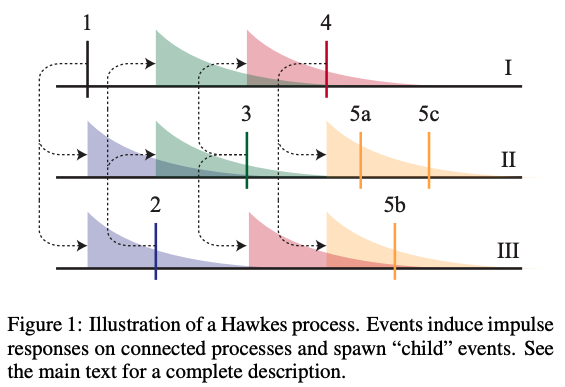
\includegraphics[width=0.6\textwidth]{17_poisson_processes//hawkes.png}
    \end{figure}
    From~\citet{linderman2014discovering}.
\end{frame}

\begin{frame}{Discovering latent network structure in point process data}
\begin{itemize}
    \itemsep1em
    
    \item We can think of the weights as defining a \textbf{directed network},
    \begin{align}
        \mbW &= 
        \begin{bmatrix}
        w_{1,1} & \ldots & w_{1,S} \\
        \vdots  &        & \vdots \\
        w_{S,1} & \ldots & w_{S,S}
        \end{bmatrix}
    \end{align}
    where $w_{s,s'} \in \reals_+$ is the strength of influence that events (points) on source $s$ induce on the intensity of source $s'$.
    
    \item However, we don't directly observe the network. We only observed it indirectly through the point process.
    
    \item \textbf{Question:} when is a multivariate Hawkes process stable, in that the intensity tends to a finite value in the infinite time limit?
\end{itemize}
\end{frame}

\begin{frame}[t]{Multivariate Hawkes processes as Poisson clustering processes}
    \begin{itemize}
        \itemsep1em
        
        \item Note that the conditional intensity in eq.~\eqref{eq:mvhawkes} is a sum of a background intensity and a bunch of non-negative impulse responses.
        \begin{align}
            \lambda_s(t \mid \cH_t) &= \lambda_{0,s} + \!\!\!\!\sum_{(t_n, s_n) \in \cH_t}\!\!\!\! h_{s_n, s}(t - t_n).
        \end{align}
        
        \item \textbf{Question:} which property of Poisson processes applied to such intensities?
    \end{itemize}
\end{frame}

\begin{frame}[t]{Multivariate Hawkes processes as Poisson clustering processes}
    \begin{itemize}
        \itemsep1em
        
        \item Note that the conditional intensity is a sum of a background intensity and a bunch of non-negative impulse responses,
        \begin{align}
            \lambda_s(t \mid \cH_t) &= \lambda_{s,0} + \!\!\!\!\sum_{(t_n, s_n) \in \cH_t}\!\!\!\! h_{s_n, s}(t - t_n).
        \end{align}
        
        \item \textbf{Question:} which property of Poisson processes applied to such intensities?
        
        \item Using the \textbf{Poisson superposition principle}, we can partition the points $\cT_s = \{t_n: s_n=s\}$ from source $s$ into \textbf{clusters} attributed to either the background or to one of the impulse responses.
        \begin{align}
            \cT_s = \bigcup_{n=0}^N \cT_{s,n}
        \end{align} 
        where
        \begin{align}
            \cT_{s,0} &\sim \mathrm{PP}(\lambda_{s,0}) & & \text{[background points]}\\ 
            \cT_{s,n} &\sim \mathrm{PP}(h_{s_n,s}(t - t_n)) & & \text{[points induced by $(t_n, s_n)$]}
        \end{align}
    \end{itemize}
\end{frame}

\begin{frame}[t]{Multivariate Hawkes processes as Poisson clustering processes}
    \begin{itemize}
        \itemsep1em
        
        \item Now the weights have an intuitive interpretation. Plugging in the definition of the impulse response,
        \begin{align}
            \cT_{s,n} &\sim \mathrm{PP}\Big(w_{s_n,s} \cdot \mathrm{Exp}(t - t_n; \tau_{s_n,s}) \Big).
        \end{align}
        \item \textbf{Question:} What is the expected number of points induced by this impulse response, i.e. $\mathbb{E}[|\cT_{s,n}|]$?
    \end{itemize}
\end{frame}

\begin{frame}[t]{Conjugate Bayesian inference for multivariate Hawkes processes}
    \begin{itemize}
        \itemsep1em
        
        \item Let's put a gamma prior on the weights, 
        \begin{align}
            w_{s,s'} &\sim \mathrm{Ga}(\alpha, \beta).
        \end{align}
        
        \item \textbf{Question:} suppose we know the partition of points; i.e. we knew the clusters~$\cT_{s,n}$. What is the conditional distribution,
        \begin{align}
            p\left(w_{s,s'} \mid \{\{\cT_{s,n}\}_{n=0}^N\}_{s=1}^S \right) &= \hspace{30em}
        \end{align}
    \end{itemize}
\end{frame}

\begin{frame}[t]{Conjugate Bayesian inference for multivariate Hawkes processes II}
    \begin{itemize}
        \itemsep1em
        
        \item We don't know the partition of spikes in general, but we do know its conditional distribution!
        
        \item Let $z_n \in \{0, \ldots, n-1\}$ denote the cluster to which the $n$-th spike is assigned, with $z_n=0$ denoting the background cluster. With this notation,
        \begin{align}
            \cT_{s,n} &= \{(t_{n'}, s_{n'}): s_{n'}=s \wedge z_{n'}=n\}.
        \end{align}
        
        \item \textbf{Question:} what is the conditional distribution of the cluster assignment,
        \begin{align}
            p(z_n \mid \{(t_n, s_n)\}_{n=1}^N; \mbtheta) &= \hspace{30em}
        \end{align}
        
        \item Using these two conditional distributions, we can derive a simple Gibbs sampling algorithm that alternates between sampling the weights given the clusters and the clusters given the weights.
    \end{itemize}
\end{frame}

\begin{frame}[t]{Beyond Poisson: Hawkes processes }
    \begin{itemize}
        \itemsep.5em
        
        \item Hawkes processes are only one way of going beyond Poisson processes. 
        
        \item Whereas Hawkes processes take an autoregressive approach, \textbf{doubly stochastic point processes} (a.k.a. \textbf{Cox processes}) take a latent variable approach.
        
        \item In these models, the intensity itself is modeled as a stochastic process,
        \begin{align}
            \lambda(\mbx) &\sim p(\lambda).
        \end{align}
        
        \item For example, consider the model,
        \begin{align}
            \lambda(\mbx) &= g(f(\mbx)) \quad \text{where} \quad
            f \sim \mathrm{GP}(\mu(\cdot), \, K(\cdot, \cdot)).
        \end{align}
        When $g$ is the exponential function, this is called a \textbf{log Gaussian Cox process}. When $g$ is the sigmoid function, this is called a \textbf{sigmoidal Gaussian Cox process}~\citep{adams2009tractable}.
        
        \item Aternatively, take $\lambda$ to be a convolution of a Poisson process with a non-negative kernel; this is called a Neyman-Scott process~\citep[e.g.]{wang2022spatiotemporal}.
    \end{itemize}
\end{frame}

\begin{frame}{Conclusion}
    \begin{itemize}
        \itemsep1em
        
        \item Poisson processes are stochastic processes that generate discrete sets of points.
        
        \item They are defined by an intensity function $\lambda(\mbx)$, which specifies the expected number of points in each interval of time or space.
        
        \item We can build in dependencies by conditioning on past points or introducing latent variables.
        
        \item Poisson process modeling boils down to inferring the intensity. We can take various parametric and nonparametric approaches.
        
        \item The hardness comes about when the integral in the Poisson process likelihood is intractable.
        
        \item As we will see next time, Poisson processes are also mathematical building blocks for Bayesian nonparametric models with random measures.
    \end{itemize}
\end{frame}

\begin{frame}[t,allowframebreaks]
        \frametitle{References}
        \bibliographystyle{unsrtnat}
        \bibliography{refs.bib}
\end{frame}

\end{document}
